\chapter{Payment Industry and Domain Analysis}\label{chap:payment-industry}
\fancyhead[R]{Payment Industry and Domain Analysis}

\textit{``This chapter provides comprehensive analysis of the payment industry ecosystem and domain fundamentals. It covers the transaction lifecycle, ecosystem participants, fee structures, messaging architectures, and current challenges in fee processing. This domain knowledge establishes the business and technical context necessary for understanding the computational challenges addressed by the P2S platform.''}

\pagebreak

\section{Introduction}

The electronic payment industry represents one of the most complex and rapidly evolving sectors in the global financial ecosystem. Understanding the intricate relationships between participants, transaction flows, fee structures, and processing architectures is essential for appreciating the technical challenges addressed by modern payment processing systems.

This chapter provides comprehensive analysis of the payment domain, focusing on the French market context while addressing the international frameworks that govern cross-border transaction processing. The analysis establishes the foundation for understanding why traditional fee calculation approaches face significant limitations and how innovative computational architectures can address these challenges.

The payment ecosystem analysis reveals fundamental complexities in fee determination that motivate the development of specialized computational engines capable of processing high-volume transaction streams while maintaining accuracy and compliance with regulatory requirements \cite{bis2018payment}.

\section{Payment Industry Overview}

The payment industry encompasses a complex ecosystem of infrastructure, institutions, and processes that facilitate monetary value transfer between transacting parties. This ecosystem operates under multiple regulatory frameworks, involves diverse stakeholder groups, and processes billions of transactions annually through sophisticated technological infrastructure.

Understanding this ecosystem is essential for appreciating the technical challenges addressed by this project, particularly the computational complexities involved in real-time fee calculation and the structural heterogeneity of payment scheme documentation.

\subsection{Industry Structure and Scale}

The global payment industry processes over 150 billion card transactions annually, with European markets accounting for approximately 25\% of this volume. The French market specifically handles over 12 billion card transactions per year, representing a significant portion of European payment activity.

This scale creates substantial computational challenges for financial institutions that must process fees for each transaction while maintaining real-time performance characteristics. The volume and velocity requirements drive the need for highly optimized processing architectures capable of handling peak transaction loads without degrading system performance.

\subsection{Regulatory Framework}

The French payment ecosystem operates within a comprehensive regulatory framework established by multiple authorities:

\begin{itemize}
    \item \textbf{European Central Bank (ECB):} Oversight of payment systems and monetary policy implementation
    \item \textbf{Banque de France:} National payment system supervision and financial stability monitoring
    \item \textbf{ACPR (Autorité de Contrôle Prudentiel et de Résolution):} Banking and insurance sector regulation
    \item \textbf{European Banking Authority (EBA):} Technical standards development and regulatory coordination
\end{itemize}

These regulatory bodies establish fee calculation requirements, interchange rate regulations, and compliance standards that directly impact the design requirements for automated fee calculation systems.

\section{Transaction Lifecycle and Processing}

Payment transactions follow a sophisticated three-phase lifecycle that involves multiple participants and complex decision-making processes. Understanding this lifecycle is crucial for designing systems that can efficiently process fees at each stage while maintaining accuracy and compliance.

\subsection{Transaction Phases}

Payment transactions follow a three-phase lifecycle that determines when and how fees are calculated and applied:

\begin{figure}[H]
    \centering
    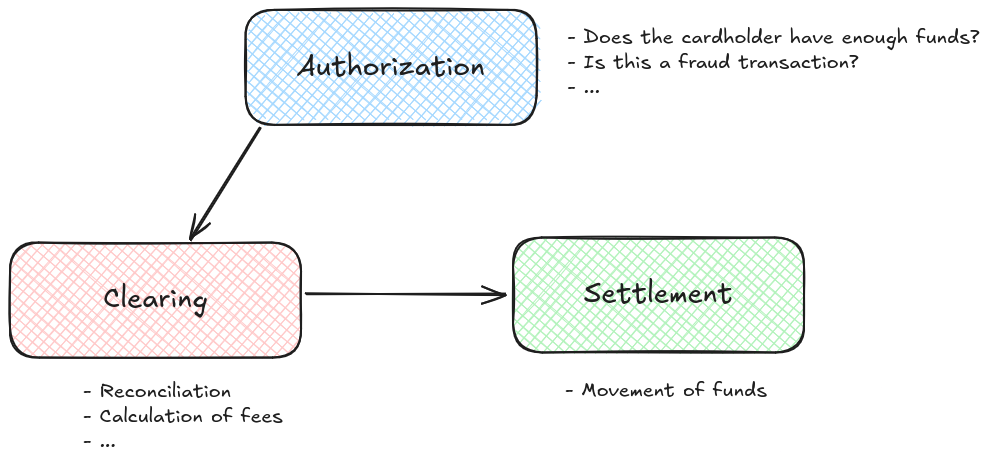
\includegraphics[width=0.8\textwidth]{img/Txn_Phases.png}
    \caption{Payment Transaction Lifecycle}
\end{figure}

\subsubsection{Authorization Phase}

The authorization phase represents the initial real-time verification of payment credentials against predetermined criteria. This phase occurs within milliseconds and involves complex decision-making algorithms that evaluate multiple risk factors:

\begin{itemize}
   \item \textbf{Account Verification:} Real-time validation of account status, available funds, and account standing
   \item \textbf{Fraud Detection:} Advanced algorithms analyzing transaction patterns and risk indicators
   \item \textbf{Regulatory Compliance:} Verification against sanctions lists and regulatory restrictions
   \item \textbf{Business Rules:} Application of issuer-specific business logic and risk management policies
\end{itemize}

Authorization processing requires sub-second response times, creating significant challenges for systems that must also calculate applicable fees during this phase.

\subsubsection{Clearing Phase}

The clearing phase encompasses the administrative processes for exchanging transaction data between participating financial institutions. This phase operates on batch processing schedules and involves comprehensive data reconciliation:

\begin{itemize}
   \item \textbf{Data Exchange:} Standardized transaction data transmission between financial institutions
   \item \textbf{Fee Calculation:} Detailed computation of interchange fees, scheme fees, and other applicable charges
   \item \textbf{Reconciliation:} Verification of transaction data accuracy and completeness
   \item \textbf{Settlement Preparation:} Generation of settlement instructions and netting calculations
\end{itemize}

The clearing phase provides the primary opportunity for detailed fee calculation and validation, making it the focus of most automated fee processing systems.

\subsubsection{Settlement Phase}

The settlement phase represents the final transfer of monetary value between financial institutions through established financial networks. This phase involves:

\begin{itemize}
   \item \textbf{Net Settlement:} Calculation of net positions between participating institutions
   \item \textbf{Funds Transfer:} Actual movement of funds through central bank or correspondent banking networks
   \item \textbf{Confirmation:} Verification of successful settlement completion
   \item \textbf{Reporting:} Generation of settlement reports and audit trails
\end{itemize}

Settlement typically occurs with delays ranging from same-day to multiple business days, depending on the specific payment network and transaction characteristics.

\subsection{Processing Complexity Factors}

Several factors contribute to the computational complexity of transaction processing:

\begin{itemize}
    \item \textbf{Volume Scalability:} Peak transaction volumes can exceed normal processing capacity by 300-400\%
    \item \textbf{Geographic Distribution:} Cross-border transactions involve multiple regulatory frameworks and currency considerations
    \item \textbf{Product Diversity:} Different card products and payment methods require specialized processing logic
    \item \textbf{Temporal Considerations:} Time-sensitive processing requirements with strict service level agreements
\end{itemize}

\section{Ecosystem Participants and Relationships}

The payment ecosystem comprises multiple specialized participants, each with distinct roles, responsibilities, and economic incentives. Understanding these relationships is essential for comprehending fee structures and the computational challenges involved in fee calculation.

\subsection{Primary Participants}

The payment ecosystem involves five primary participant categories:

\begin{itemize}
   \item \textbf{Consumer:} Transaction initiator using payment credentials linked to accounts at issuing institutions
   \item \textbf{Merchant:} Commercial entity accepting payment for goods or services
   \item \textbf{Issuer:} Financial institution responsible for credential issuance and consumer account maintenance
   \item \textbf{Acquirer:} Financial institution providing payment acceptance services to merchants
   \item \textbf{Card Network:} Infrastructure provider establishing connectivity between issuers and acquirers
\end{itemize}

\begin{figure}[H]
    \centering
    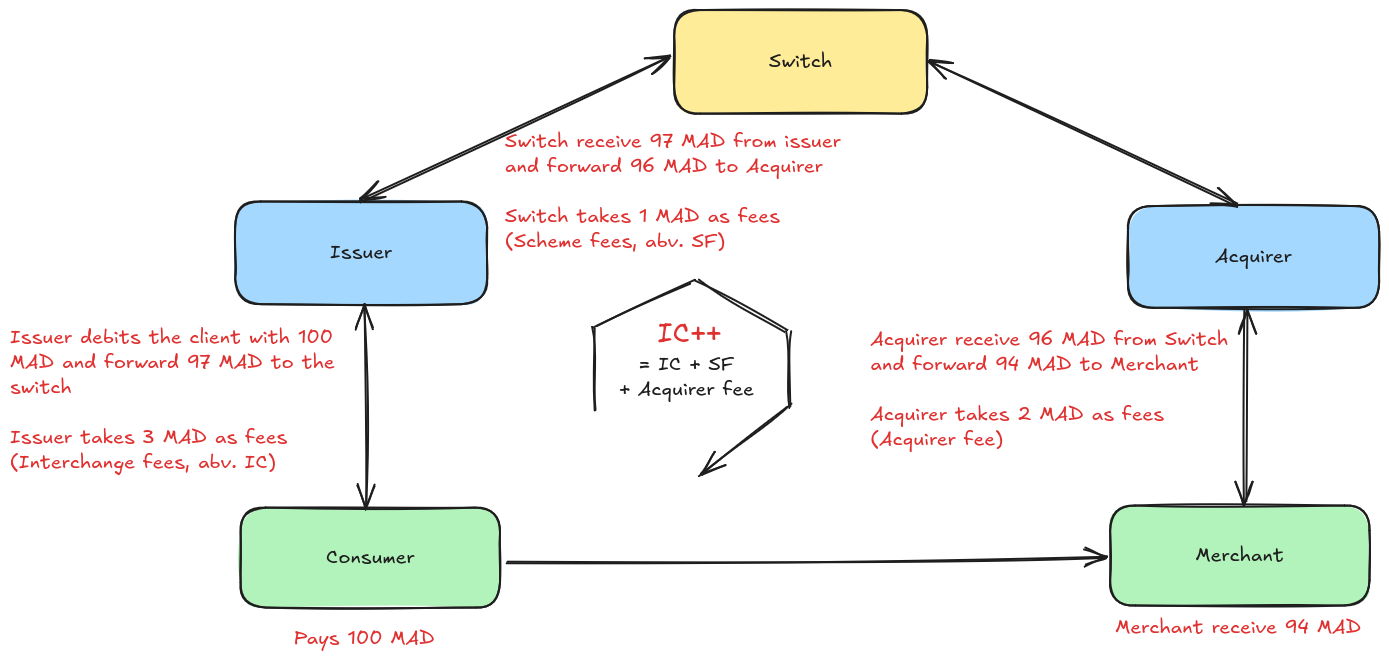
\includegraphics[width=\textwidth]{img/Txn_Actors.png}
    \caption{Payment Ecosystem Participants and Fee Flow}
\end{figure}

\subsection{Issuer Role and Responsibilities}

Issuers represent the financial institutions that establish relationships with consumers and maintain their payment accounts. Key responsibilities include:

\begin{itemize}
    \item \textbf{Account Management:} Maintaining consumer payment accounts and credit facilities
    \item \textbf{Risk Management:} Evaluating and managing credit risk for account holders
    \item \textbf{Fraud Prevention:} Implementing systems to detect and prevent fraudulent transactions
    \item \textbf{Regulatory Compliance:} Ensuring compliance with consumer protection and financial regulations
    \item \textbf{Fee Collection:} Collecting interchange fees from acquirers for transaction processing
\end{itemize}

Issuers face complex fee calculation challenges due to the variety of interchange structures and bilateral agreements that may apply to different transaction types.

\subsection{Acquirer Role and Responsibilities}

Acquirers provide payment acceptance infrastructure for merchants and handle the complexity of connecting to multiple payment networks. Key responsibilities include:

\begin{itemize}
    \item \textbf{Merchant Services:} Providing payment acceptance technology and services to commercial entities
    \item \textbf{Transaction Processing:} Routing transactions through appropriate payment networks
    \item \textbf{Risk Management:} Managing merchant-related risks and chargebacks
    \item \textbf{Settlement Services:} Facilitating settlement of funds to merchant accounts
    \item \textbf{Fee Payment:} Paying interchange fees to issuers and scheme fees to payment networks
\end{itemize}

Acquirers must manage complex fee structures that vary based on merchant type, transaction characteristics, and payment network requirements.

\subsection{Payment Network Role and Responsibilities}

Payment networks (such as Visa and Mastercard) provide the technological infrastructure and regulatory framework for transaction processing. Key responsibilities include:

\begin{itemize}
    \item \textbf{Network Infrastructure:} Operating the technical infrastructure for transaction routing and processing
    \item \textbf{Standards Development:} Establishing technical and business standards for network participants
    \item \textbf{Rule Enforcement:} Ensuring compliance with network rules and regulations
    \item \textbf{Fraud Prevention:} Operating network-level fraud detection and prevention systems
    \item \textbf{Fee Management:} Establishing and collecting scheme fees from network participants
\end{itemize}

Payment networks establish complex fee structures that create significant computational challenges for automated processing systems.

\section{Fee Structures and Economic Models}

The payment ecosystem operates on sophisticated multi-party fee structures that create complex computational challenges for automated processing systems. Understanding these fee structures is essential for appreciating the technical requirements of modern fee calculation engines.

\subsection{Multi-Party Fee Structure}

The payment ecosystem operates on a multi-party fee structure that involves multiple concurrent fee calculations:

\begin{itemize}
   \item \textbf{Interchange Fee:} Compensation from acquirers to issuers for each transaction, incentivizing credential issuance and compensating for credit risk
   \item \textbf{Scheme Fee:} Compensation to card networks for infrastructure services, financing network operations and fraud detection systems
   \item \textbf{Acquirer Fee:} Compensation retained by acquirers for merchant services, covering processing costs and risk management
\end{itemize}

Each fee type involves distinct calculation methodologies, qualification criteria, and regulatory constraints that must be evaluated simultaneously for each transaction.

\subsection{Interchange Fee Structures}

Interchange fees represent the most complex component of payment processing costs due to their multi-dimensional qualification criteria and regulatory constraints.

\subsubsection{Qualification Dimensions}

Interchange fee determination involves evaluation of multiple transaction characteristics:

\begin{itemize}
    \item \textbf{Geographic Factors:} Issuer and acquirer locations, cross-border transaction status
    \item \textbf{Merchant Classification:} Merchant Category Code (MCC) and business type
    \item \textbf{Card Product Type:} Credit, debit, commercial, premium card classifications
    \item \textbf{Transaction Channel:} Online, in-store, mobile, contactless payment methods
    \item \textbf{Processing Method:} Chip, magnetic stripe, contactless, manual processing
    \item \textbf{Authentication Status:} PIN verification, signature, biometric authentication
\end{itemize}

\subsubsection{Regulatory Constraints}

European interchange fee regulations impose specific constraints on fee calculations:

\begin{itemize}
    \item \textbf{Consumer Card Caps:} Maximum 0.2\% for debit cards, 0.3\% for credit cards
    \item \textbf{Commercial Card Regulations:} Separate regulatory framework for business cards
    \item \textbf{Cross-Border Transactions:} Specific rules for transactions crossing European borders
    \item \textbf{Three-Party Scheme Rules:} Different regulations for schemes like American Express
\end{itemize}

\subsection{Scheme Fee Structures}

Payment schemes employ sophisticated fee structures that vary significantly between networks and evolve frequently based on business strategy and competitive dynamics.

\subsubsection{Cost Code Methodologies}

Scheme fees typically employ cost code systems that categorize transactions into fee categories:

\begin{itemize}
    \item \textbf{Hierarchical Classification:} Multi-level categorization based on transaction attributes
    \item \textbf{Volume Thresholds:} Progressive fee structures based on institutional transaction volumes
    \item \textbf{Service-Specific Fees:} Specialized fees for premium services and enhanced processing
    \item \textbf{Promotional Structures:} Temporary fee adjustments for market development initiatives
\end{itemize}

\subsubsection{Fee Calculation Complexity}

Scheme fee calculation involves multiple computational challenges:

\begin{itemize}
    \item \textbf{Rule Priority Resolution:} Determining which fee rules apply when multiple rules match
    \item \textbf{Temporal Considerations:} Applying time-sensitive promotional rates and volume thresholds
    \item \textbf{Currency Conversion:} Handling multi-currency transactions and conversion rates
    \item \textbf{Aggregation Logic:} Combining multiple fee components into final scheme fee amounts
\end{itemize}

\section{Messaging Architectures and Technical Infrastructure}

Payment processing systems employ sophisticated messaging architectures that determine how transaction data flows through the ecosystem and when fee calculations are performed.

\subsection{Messaging System Types}

Two principal messaging architectures are employed in modern payment processing:

\begin{figure}[H]
    \centering
    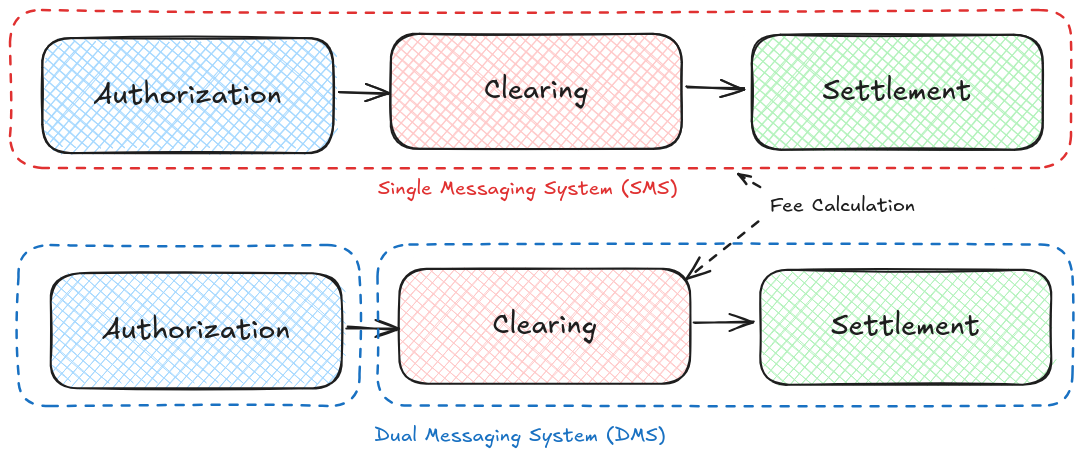
\includegraphics[width=0.8\textwidth]{img/Txn_SMS_DMS.png}
    \caption{Single and Dual Messaging Systems}
\end{figure}

\subsubsection{Single Messaging System (SMS)}

Single Messaging Systems process authorization, clearing, and settlement through unified communication pathways:

\begin{itemize}
   \item \textbf{Real-Time Processing:} All transaction phases processed concurrently
   \item \textbf{Simplified Architecture:} Reduced system complexity through unified processing
   \item \textbf{Limited Flexibility:} Constraints on complex transaction scenarios
   \item \textbf{Performance Optimization:} Streamlined processing for high-volume environments
\end{itemize}

SMS architectures create specific challenges for fee calculation systems that must operate within strict real-time performance constraints.

\subsubsection{Dual Messaging System (DMS)}

Dual Messaging Systems separate authorization and clearing phases, enabling more sophisticated processing:

\begin{itemize}
   \item \textbf{Phase Separation:} Independent processing of authorization and clearing phases
   \item \textbf{Enhanced Flexibility:} Support for complex transaction scenarios and delayed settlement
   \item \textbf{Detailed Processing:} Comprehensive data exchange and validation capabilities
   \item \textbf{Fee Calculation Optimization:} Enhanced opportunities for detailed fee computation
\end{itemize}

DMS architectures provide more opportunities for sophisticated fee calculation but require more complex system integration.

\subsection{Technical Standards and Protocols}

Payment processing systems operate according to established technical standards that define message formats, processing requirements, and integration specifications.

\subsubsection{ISO Standards}

International Organization for Standardization (ISO) standards provide the foundation for payment message processing:

\begin{itemize}
    \item \textbf{ISO 8583:} Financial transaction card originated messages standard
    \item \textbf{ISO 20022:} Universal financial industry message scheme
    \item \textbf{ISO 27001:} Information security management systems requirements
    \item \textbf{ISO 9001:} Quality management systems requirements
\end{itemize}

\subsubsection{Network-Specific Standards}

Individual payment networks establish proprietary standards that extend ISO requirements:

\begin{itemize}
    \item \textbf{Visa Standards:} VisaNet processing requirements and message specifications
    \item \textbf{Mastercard Standards:} Mastercard network processing rules and technical specifications
    \item \textbf{Regional Standards:} European and French market-specific requirements
    \item \textbf{Security Standards:} PCI DSS and other security framework requirements
\end{itemize}

\section{Current Challenges in Fee Processing}

Contemporary payment processing systems face significant challenges in fee calculation and management that motivate the development of advanced computational architectures.

\subsection{Structural Complexity Challenges}

The fundamental challenge in automated fee processing stems from the structural complexity of payment scheme documentation and rule specification.

\subsubsection{Documentation Heterogeneity}

Payment schemes distribute fee specifications through inconsistent documentation formats that create significant processing challenges:

\begin{itemize}
    \item \textbf{Format Diversity:} PDF documents, spreadsheets, and proprietary formats
    \item \textbf{Structural Inconsistency:} Varying organization and presentation approaches
    \item \textbf{Embedded Logic:} Natural language expressions of conditional fee logic
    \item \textbf{Cross-References:} Complex interdependencies between document sections
    \item \textbf{Update Frequency:} Regular changes requiring system updates and validation
\end{itemize}

These documentation challenges necessitate significant manual intervention and create ongoing maintenance overhead for automated systems.

\subsubsection{Rule Complexity}

Fee determination rules exhibit multiple dimensions of complexity that challenge traditional processing approaches:

\begin{itemize}
    \item \textbf{Multi-Dimensional Qualification:} Rules depend on numerous transaction attributes
    \item \textbf{Hierarchical Structures:} Complex rule hierarchies with priority resolution requirements
    \item \textbf{Temporal Dependencies:} Time-sensitive rules and promotional rate structures
    \item \textbf{Conditional Logic:} Complex if-then logic embedded in natural language descriptions
    \item \textbf{Exception Handling:} Special cases and override conditions that require careful processing
\end{itemize}

\subsection{Computational Limitations}

Traditional fee calculation systems demonstrate significant computational limitations that impact operational efficiency and scalability.

\subsubsection{Performance Degradation}

Current systems exhibit performance characteristics that degrade as rule complexity increases:

\begin{itemize}
   \item \textbf{Linear Scaling Issues:} Processing time increases linearly with rule complexity
   \item \textbf{Resource Contention:} Shared processing resources create bottlenecks during peak periods
   \item \textbf{Memory Limitations:} Large rule sets exceed available memory for efficient processing
   \item \textbf{Network Latency:} Distributed processing creates communication overhead
\end{itemize}

\subsubsection{Architectural Constraints}

Monolithic system architectures create fundamental limitations for scalable fee processing:

\begin{itemize}
   \item \textbf{Scalability Constraints:} Inability to scale individual components based on processing requirements
   \item \textbf{Fault Isolation:} System failures impact entire processing pipeline
   \item \textbf{Deployment Complexity:} Changes require full system deployment and testing
   \item \textbf{Technology Constraints:} Difficulty adopting new technologies and processing approaches
\end{itemize}

\subsection{Operational Impact}

These technical challenges create measurable operational impacts for financial institutions:

\subsubsection{Cost Implications}

\begin{itemize}
   \item \textbf{Infrastructure Costs:} Over-provisioning of computational resources to handle peak loads
   \item \textbf{Maintenance Overhead:} Significant manual effort required for rule updates and system maintenance
   \item \textbf{Operational Costs:} Manual validation processes and error correction procedures
   \item \textbf{Opportunity Costs:} Inability to implement advanced fee optimization strategies
\end{itemize}

\subsubsection{Risk Factors}

\begin{itemize}
   \item \textbf{Compliance Risk:} Higher probability of fee calculation errors and regulatory violations
   \item \textbf{Operational Risk:} System failures during peak processing periods
   \item \textbf{Competitive Risk:} Inability to adapt quickly to market changes and competitive dynamics
   \item \textbf{Technical Risk:} Legacy system limitations and technological obsolescence
\end{itemize}

\section{Market Dynamics and Evolution}

The payment industry continues to evolve rapidly, driven by technological innovation, regulatory changes, and shifting consumer preferences. Understanding these dynamics is essential for designing systems that can adapt to future requirements.

\subsection{Technological Trends}

Several technological trends are reshaping the payment processing landscape:

\begin{itemize}
    \item \textbf{Real-Time Processing:} Increasing demand for instant payment processing and settlement
    \item \textbf{API-First Architecture:} Shift toward microservices and API-based system integration
    \item \textbf{Cloud Infrastructure:} Migration to cloud-based processing and storage solutions
    \item \textbf{Artificial Intelligence:} Application of AI for fraud detection and process optimization
    \item \textbf{Blockchain Technology:} Exploration of distributed ledger technologies for payment processing
\end{itemize}

\subsection{Regulatory Evolution}

The regulatory landscape continues to evolve with implications for fee processing systems:

\begin{itemize}
    \item \textbf{Open Banking:} Requirements for API access and data sharing
    \item \textbf{Digital Currency:} Regulatory frameworks for central bank digital currencies
    \item \textbf{Cross-Border Payments:} Enhanced requirements for international transaction processing
    \item \textbf{Data Protection:} Strengthened privacy requirements and data governance standards
\end{itemize}

\section{Chapter Conclusion}

This chapter has provided comprehensive analysis of the payment industry ecosystem, establishing the domain knowledge necessary for understanding the computational challenges addressed by the P2S platform. The analysis reveals the fundamental complexity of modern payment processing and the specific challenges that motivate the development of advanced fee calculation systems.

The payment ecosystem's multi-party structure, complex fee determination requirements, and high-volume processing demands create significant computational challenges that traditional monolithic architectures cannot efficiently address. The structural heterogeneity of payment scheme documentation and the computational limitations of current systems directly impact operational efficiency and create substantial cost and compliance risks for financial institutions.

The technical infrastructure analysis demonstrates the importance of sophisticated messaging architectures and the opportunities that modern event-driven systems provide for optimized fee processing. The dual messaging system architecture, in particular, enables the separation of real-time authorization processing from detailed fee calculation, creating opportunities for specialized computational engines.

Understanding these domain fundamentals provides the foundation for appreciating how the P2S compute engines address these challenges through stateless, event-driven architecture designed for high-performance fee calculation. The next chapter will examine existing solutions and establish the theoretical foundations for the proposed computational architecture.